\documentclass[10pt]{article}


\usepackage{times}
\usepackage{amsfonts}
\usepackage{amsmath}
\usepackage[psamsfonts]{amssymb}
\usepackage{latexsym}
\usepackage{color}
\usepackage{graphics}
\usepackage{enumerate}
\usepackage{amstext}
\usepackage{blkarray}
\usepackage{url}
\usepackage{epsfig}
\usepackage{bm}
\usepackage{hyperref}
\hypersetup{
    colorlinks=true,
    linkcolor=blue,
    filecolor=magenta,      
    urlcolor=blue,
}
\usepackage{mathtools}
\usepackage{minted}
 
\def\Kset{\mathbb{K}}
\def\Nset{\mathbb{N}}
\def\Qset{\mathbb{Q}}
\def\Rset{\mathbb{R}}
\def\Sset{\mathbb{S}}
\def\Zset{\mathbb{Z}}
\def\squareforqed{\hbox{\rlap{$\sqcap$}$\sqcup$}}
\def\qed{\ifmmode\squareforqed\else{\unskip\nobreak\hfil
\penalty50\hskip1em\null\nobreak\hfil\squareforqed
\parfillskip=0pt\finalhyphendemerits=0\endgraf}\fi}

\DeclareMathOperator*{\E}{\rm E}
\DeclareMathOperator*{\argmax}{\rm argmax}
\DeclareMathOperator*{\argmin}{\rm argmin}
\DeclareMathOperator{\sgn}{sign}
\DeclareMathOperator{\supp}{supp}
\DeclareMathOperator{\last}{last}
\DeclareMathOperator{\sign}{\sgn}
\DeclareMathOperator{\diag}{diag}
\providecommand{\abs}[1]{\lvert#1\rvert}
\providecommand{\norm}[1]{\lVert#1\rVert}
\def\vcdim{\textnormal{VCdim}}
\DeclareMathOperator*{\B}{\textbf{B}}
\DeclarePairedDelimiter\ceil{\lceil}{\rceil}
\DeclarePairedDelimiter\floor{\lfloor}{\rfloor}

\newcommand{\cX}{{\mathcal X}}
\newcommand{\cY}{{\mathcal Y}}
\newcommand{\cA}{{\mathcal A}}
\newcommand{\ignore}[1]{}
\newcommand{\bi}{\begin{itemize}}
\newcommand{\ei}{\end{itemize}}
\newcommand{\be}{\begin{enumerate}}
\newcommand{\ee}{\end{enumerate}}
\newcommand{\bd}{\begin{description}}
\newcommand{\ed}{\end{description}}
\newcommand{\h}{\widehat}
\newcommand{\e}{\epsilon}
\newcommand{\mat}[1]{{\mathbf #1}}
\newcommand{\R}{\mat{R}}
\newcommand{\0}{\mat{0}}
\newcommand{\M}{\mat{M}}

\newcommand{\SP}{\mathbf{S}_{+}^n}

\newcommand{\D}{\mat{D}}
\renewcommand{\r}{\mat{r}}
\newcommand{\x}{\mat{x}}
\renewcommand{\u}{\mat{u}}
\renewcommand{\v}{\mat{v}}
\newcommand{\w}{\mat{w}}
\renewcommand{\H}{\text{0}}
\newcommand{\T}{\text{1}}
\newcommand{\set}[1]{\{#1\}}
\newcommand{\xxi}{{\boldsymbol \xi}}
\newcommand{\ssigma}{{\boldsymbol \sigma}}
\newcommand{\Alpha}{{\boldsymbol \alpha}}
\newcommand{\tts}{\tt \small}
\newcommand{\hint}{\emph{hint}}
\newcommand{\matr}[1]{\bm{#1}}     % ISO complying version
\newcommand{\vect}[1]{\bm{#1}}     % ISO complying version

\newcommand{\Var}{\mathrm{Var}}
\newcommand{\Cov}{\mathrm{Cov}}

% New commands
\newcommand{\dom}{\textbf{dom}}
\newcommand{\epi}{\textbf{epi}}

\newenvironment{solution}{\vspace{.25cm}\noindent{\it Solution:}}{}

\begin{document}


\noindent MATH-GA.2012.001 Selected Topics in Numerical Analysis :\\
Convex and Nonsmooth Optimization, Spring 2020\\
Homework Assignment 2 \\
Yves Greatti - yg390\\

\begin{enumerate}

\item Prove that a function is convex if and only if its epigraph is a convex set. 
Suppose $f$ is a convex function, $f: \mathbf{R}^n \rightarrow \mathbf{R}$ then $\forall (x, t_1),(y, t_2) \in \epi f$, and $\forall  \theta \in [0, 1]$,
we want to show that $\theta (x, t_1) + (1-\theta) (y, t_2)$ is in $\epi f$.
we have:
\begin{align*}
	f(\theta x + (1-\theta) y)	&\le	\theta f(x) + (1 - \theta) f(y) \\
						&\le	\theta t_1 + (1 - \theta) t_2
\end{align*} thus $\epi f$ is convex. The other direction is similar  $\forall (x, t_1),(y, t_2) \in \epi f$, $\epi f$ is a convex set, and $\forall  \theta \in [0, 1]$:
Let $t_1 = f(x)$, $t_2 = f(y)$ thus $\theta (x, t_1) + (1-\theta) (y, t_2) = (\theta x + (1-\theta) y, \theta t_1 + (1-\theta) t_2)$ is in $\epi f$ which implies: 
$f(\theta x + (1-\theta) y) \le \theta t_1 + (1-\theta) t_2 \Rightarrow$  $f(\theta x + (1-\theta) y) \le \theta f(x) + (1-\theta) f(y) \Rightarrow f$ is convex.

\item BV Ex. 2.31 Properties of dual cones. Let $K^*$ be the dual cone of a convex cone K. Prove the following.
	\be 
		\item $K^*$  is indeed a convex cone.
		$\forall y_1, y_2  \in K^*, \theta_1, \theta_2 \ge 0$, and $\forall x \in K$, 
		$x^T (\theta_1 y_1 + \theta_2 y_2) = \theta_1 x^T y_1 + \theta_2 x^T y_2 \ge 0$ thus $K^*$ is a convex cone.
		
		\item $K_1 \subseteq K_2$ implies $K_2^* \subseteq K_1^*$.
		Suppose $y \in K_2^*$, $\forall x \in K_1$, $x^T y \ge 0$, and since $x \in K_2$ also, then $y \in K_1^*$ and $K_2^* \subseteq K_1^*$.
	\ee
	
\item Show that if a convex cone K is closed, then $(K^*)^*$, the dual cone of the dual cone of K, is equal to K.
source: class notes on the web pointing that $(K^*)^*$ can be seen as the intersection of halfspaces.

Let K a convex closed cone, then $(K^*)^* = \{x^* | y^T x^* \ge 0, \forall y \in K^* \}$.  We can consider $(K^*)^*$ as the intersection of halfspaces $H_{x^* \in K} = \{y^T x^* \ge 0, \forall y \in K^* \}$. If $x \in K$ then $\forall y \in K^*, x^T y = y^T x \ge 0 \Rightarrow x \in (K^*)^*$. K being convex and closed by the corollary of the separating hyperplanes, $K = (K^*)^*$.

\item BV Ex. 233 Find the dual cone of $\{ A \; x | x \ge 0 \}$, where $A \in \mathbf{R}^{m \times n}$. 
The dual of $K = \{ A \; x | x \ge 0 \}$ is $K^* = \{ y | (A x)^T y \ge 0, \forall x \ge 0 \}$ or $K^* = \{ y | x^T (A^T y) \ge 0,  x \ge 0 \} = \{ y | (A^T y)^T x \ge 0, x \ge 0 \}$. 
Given $u = A^T y$, we are looking for vectors $u$ such that the inner product is non-negative for any $x \ge 0$.
Let $\{e_1, \cdots  ,e_n\}$ the canonical basis for $\mathbf{R}^n$, for any vector $u = A^T y, y \in K^*$, we have $u^T e_i \ge 0 \Rightarrow u_i \ge 0, i \in [1,n]$.
Thus $K^* = \{ y | A^T y \ge 0, x \ge 0\}$, this is sufficient as if $ x\ge 0$ then $x^T  A^T y \ge 0$.
	
\item Show that the second-order cone defined on p.31 of BV is self-dual, that is, it satisfies $K^* = K$.
Let C the second-order cone, $C=\{(x, t) \in  \mathbf{R}^n | \| x \|_2 \le t \}$. $C^* = \{(y,s) | \begin{bmatrix} x \\ t  \end{bmatrix}^T \begin{bmatrix} y \\ s  \end{bmatrix} \ge 0, \forall (x,t) \in C\}$.
if $(y, s) \in C$ then $x^T y \le \| x \|_2 \| y \|_2$ using Cauchy-Schwarz or  $x^T y \le t \; s$. 
$\begin{bmatrix} x \\ t  \end{bmatrix}^T \begin{bmatrix} y \\ s  \end{bmatrix}  = x^T y + ts$, and by the triangle inequality, $\|x^T y + ts\|  \ge t \; s - | x^T y | \ge 0 \Rightarrow y \in C^*$.
Suppose $(y, s) \notin C$, then $\| y \|_2 > s$ and let m the index of the largest component of $y$, 
thus $\| y \|_2 = (\sum_{i=1,n} y_i^2)^{\frac{1}{2}} \le (n^2 |y_m|^2)^{\frac{1}{2}} = n |y_m| \Rightarrow $. WLOG $| y_m | = y_m$, then $y_m > \frac{n} {s^2}$
and let $x$ the vector with the only component non-zero $x_m = - \frac{n} {s^2}$ then $x^T y = - \frac{n} {s^2} \; y_m \le - 1$ so $y \notin C^*$.
In conclusion, $C = C^*$, C is self-dual.
 
\item  "Chebyshev center" problem

\begin{enumerate}
\item function  chebyshev\_center(A, b) takes a matrix $A$ of dimension $(2,n)$ and a vector $b(n)$ to find the  largest Euclidean ball
that lies in a polyhedron described by $n$ linear inequalities.
 
\begin{minted}{matlab}

% Compute the Chebyshev center of a polyhedron
% Boyd & Vandenberghe "Convex Optimization"
function [x_sol, r_sol] = chebyshev_center(A, b)
% The goal is to find the largest Euclidean ball (i.e. its center and
% radius) that lies in a polyhedron described by linear inequalites in this
% fashion: P = {x : a_i'*x <= b_i, i=1,...,m}

% Generate the data
[~,n]=size(A);

% Build and execute model
fprintf(1,'Computing Chebyshev center...');
cvx_begin
    variable r(1)
    variable x_c(2)
    maximize ( r )
    for k=1:n
        A(:, k)'*x_c + r*norm(A(:, k),2) <= b(k);
    end
cvx_end
fprintf(1,'Done! \n');
x_sol = x_c;
r_sol = r;

% Display results
fprintf(1,'The Chebyshev center coordinates are: \n');
disp(x_c);
fprintf(1,'The radius of the largest Euclidean ball is: \n');
disp(r);

% Generate the figure
x = linspace(-2,2);
for k=1:n
    plot(x, -x * A(1,k)./A(2,k) + b(k)./A(2,k),"b-");
    hold on
end
theta = 0:pi/100:2*pi;
plot( x_c(1) + r*cos(theta), x_c(2) + r*sin(theta), "r" );
plot(x_c(1),x_c(2),'b*');
xlabel("x_1")
ylabel("x_2")

txt = "# inequalities:" + num2str(n);
title({"Largest Euclidean ball laying in a 2D polyhedron", txt});
text(x_c(1), x_c(2), "\leftarrow  center")
axis([-1 1 -1 1])
axis equal
hold off
txt = "chebyshev_center_" + num2str(n);
saveas(gcf,txt,'epsc')

\end{minted}

For the same example on the web page where matrix $A=\begin{bmatrix} 2 &  2  & -1 & -1\\ 1 & -1 & 2  & -2 \end{bmatrix}$ and vector $b=\begin{bmatrix} 1\\ 1 \\ 1 \\ 1 \end{bmatrix}$,
we obtain the same circle which is tangent to the four hyperplanes $a_i^T x = b_i$ (see figure ~\ref{fig1}):
\begin{figure}[H]
	\centering
	%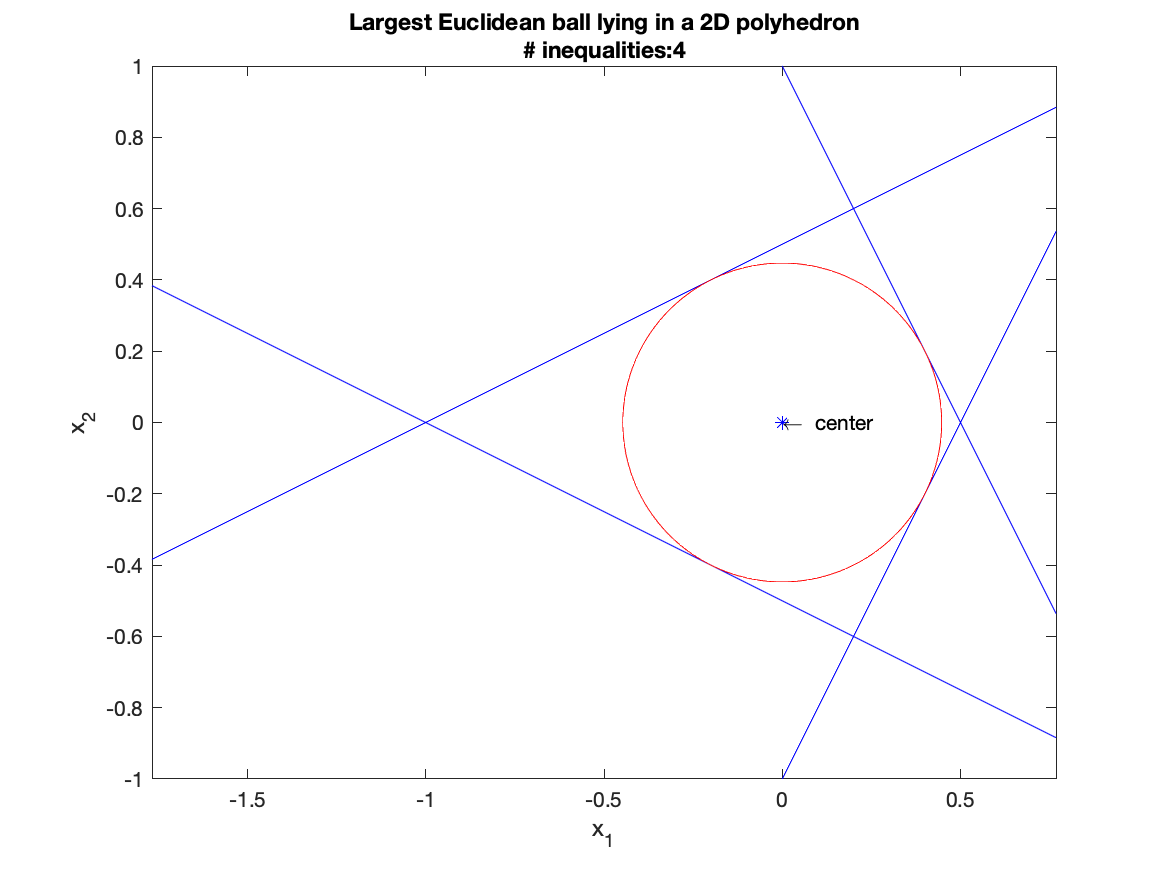
\includegraphics[width=1\linewidth]{figures/chebyshev_center_4} 
	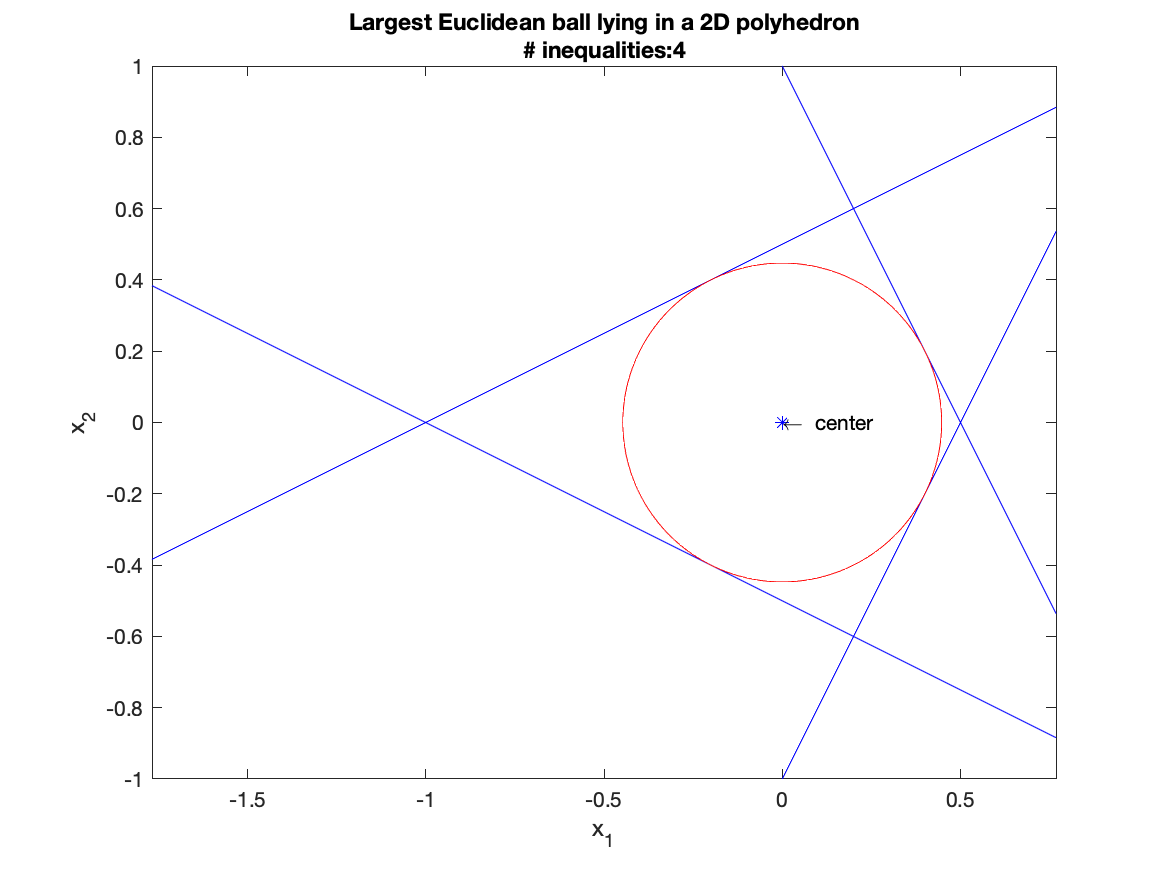
\includegraphics[width=200pt]{figures/chebyshev_center_4}
	\caption{Sample example}
	\label{fig1}
\end{figure}
     

We solve the same optimization problem with more inequalities and an interior center inside the polyhedron (see figure ~\ref{fig2}):
\begin{figure}[H]
	\centering
	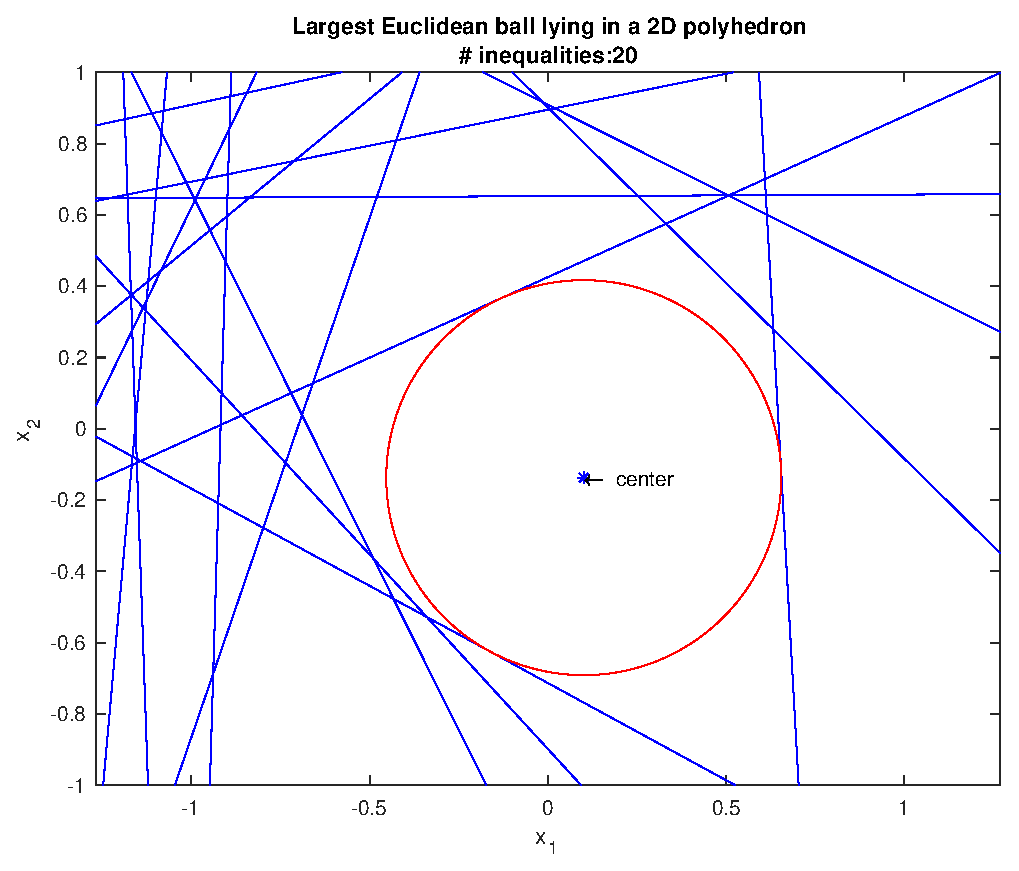
\includegraphics[width=200pt]{figures/chebyshev_center_20}
	\caption{Example with 20 inequalities}
	\label{fig2}
\end{figure}

\item If we choose A and b such that there is no interior point : if the hyperplanes intersect at the same point then CVX finds a center with radius zero, if they do not intersect then CVX will not find a solution.

\item The problem to solve now is to find the largest "scaled unit ball" $\mathcal{B} = \{x_c + u | \| u \|_p \le r \}$ that lies in the polyhedron described by a set of linear inequalities:
$\mathcal{P} = \{x \in \mathbf{R}^n | a_i^T x \le b_i, i=1, \cdots, m \}$. For any point of $\mathcal{B}$ laying in one halfspace $a_i^T x \le b_i$, similarly to the euclidean space, 
we have $\| u \|_p \le r \Rightarrow a_i^T x_c +  r \| a_i \|_p  \le b_i$ since $g_i = \sup{\{a_i^T u | \| u \|_p \le r \}} = r \|a_i\|_p$. And the Chebyshev center can be determined by solving the problem:
\begin{align*}
	\text{ maximize } &  r\\
	\text{subject to }  & a_i^T x_c +  r \| a_i \|_p  \le b_i,  i=1, \cdots, m
\end{align*}
This is still an LP problem since the inequalities are linear.
We obtain different solutions for the same matrix $A$ and vector $b$, corresponding to different p-norm, $p=1$ is the diamond shape ball (fig.  ~\ref{fig3}),
for $p=1.5$  the ball has a shape between the diamond and the circle $p=2$ (fig. ~\ref{fig4}), and as we increase $p$, for $p=\infty$ the ball becomes a square 
(where either $\|x\| =1 \text{ and } \| y \| \le 1 \text{ or } \| x \| \le 1 \text{ and } \| y || = 1$,  (fig. ~\ref{fig5})).

\begin{figure}[H]
	\centering
	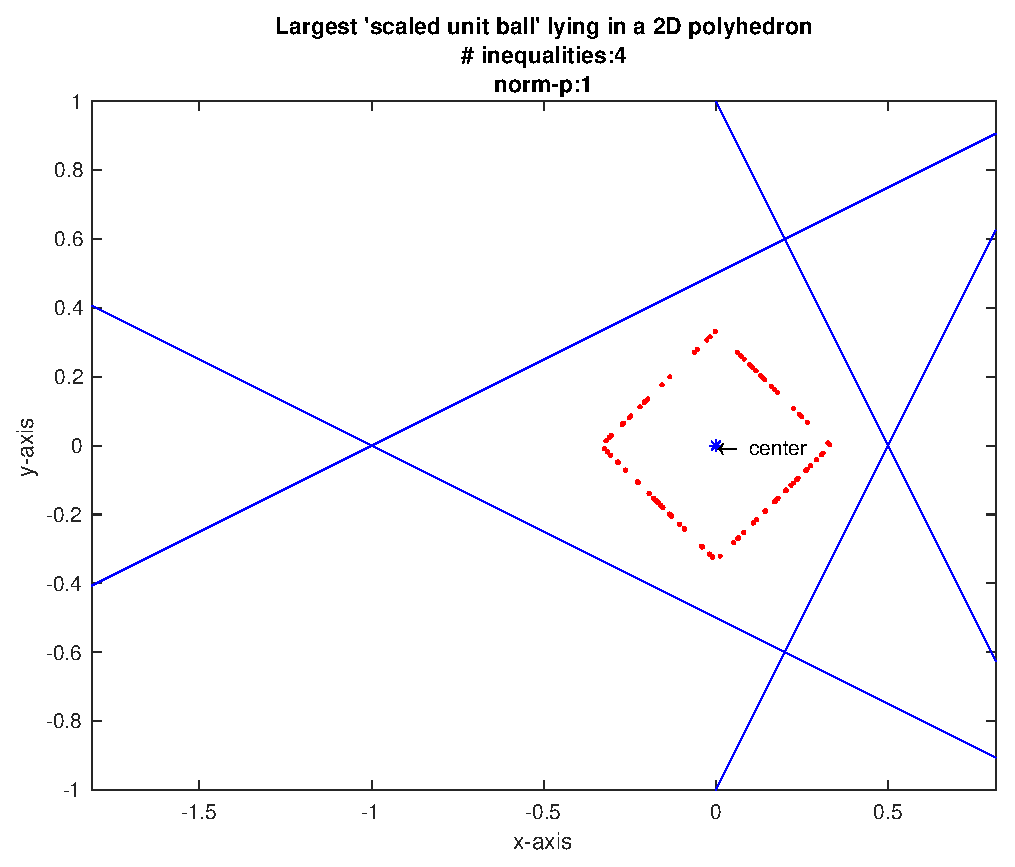
\includegraphics[width=200pt]{figures/chebyshev_center_norm_1}
	\caption{"Scaled" unit ball for p=1}
	\label{fig3}
\end{figure}
\begin{figure}[H]
	\centering
	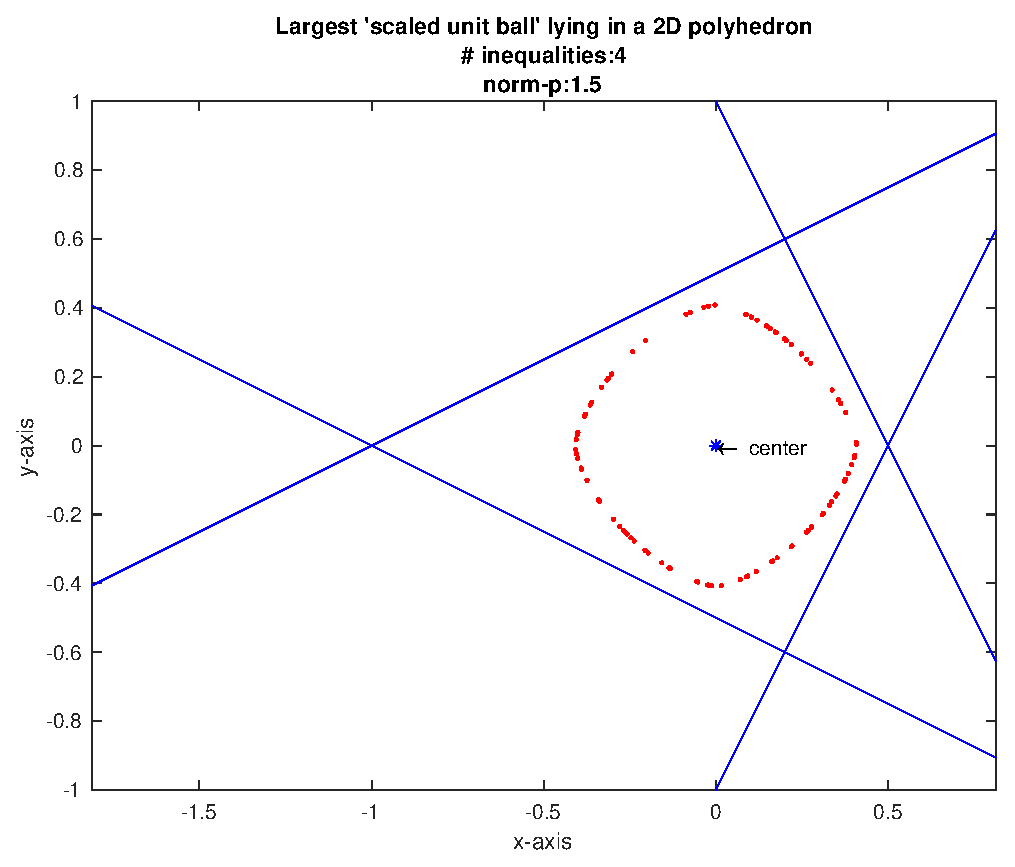
\includegraphics[width=200pt]{figures/chebyshev_center_norm_15}
	\caption{"Scaled" unit ball for p=1.5}
	\label{fig4}
\end{figure}
\begin{figure}[H]
	\centering
	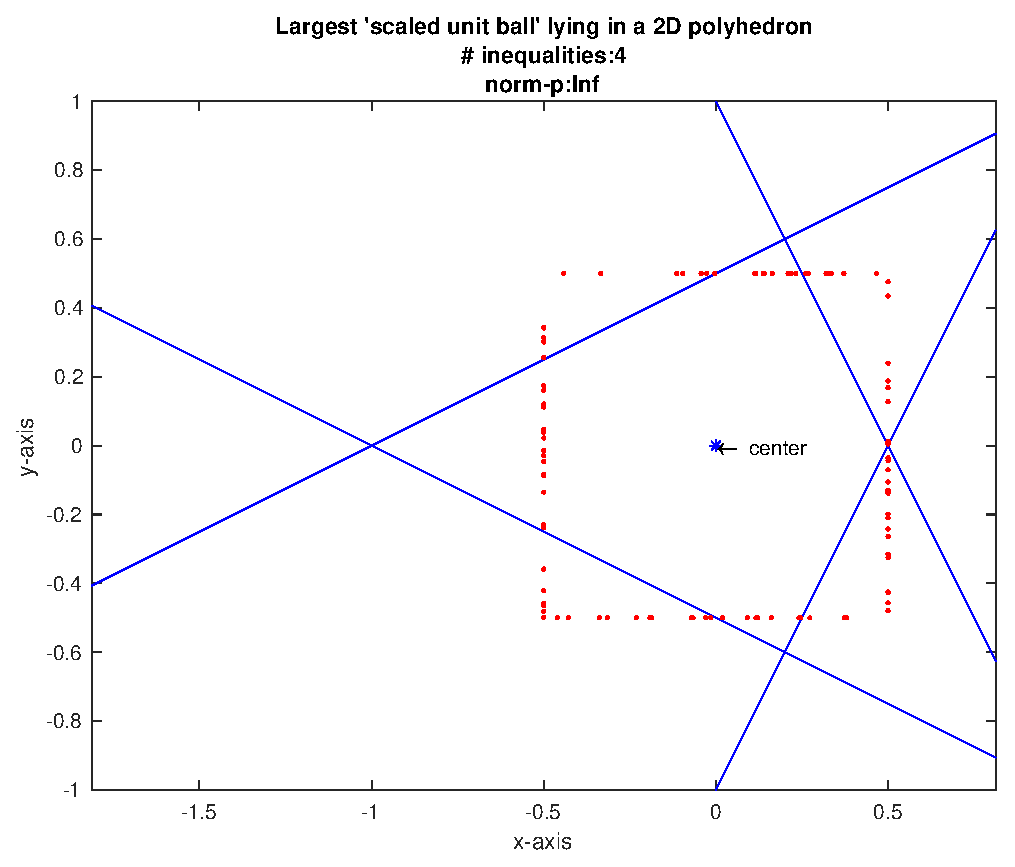
\includegraphics[width=200pt]{figures/chebyshev_center_norm_Inf}
	\caption{"Scaled" unit ball for p=$\infty$}
	\label{fig5}
\end{figure}

\begin{minted}{matlab}

% Compute the Chebyshev center of a polyhedron
function [x_sol, r_sol] = chebyshev_center_with_norm(A, b, p)
% The goal is to find the largest Euclidean ball (i.e. its center and
% radius) that lies in a polyhedron described by linear inequalites in this
% fashion: P = {x : a_i'*x <= b_i, i=1,...,m}

rng('default')
format long g
[~,n]=size(A);

% Build and execute model
fprintf(1,'Computing Chebyshev center...');
cvx_begin
    variable r(1)
    variable x_c(2)
    maximize ( r )
    for k=1:n
        A(:, k)' * x_c + r * norm(A(:, k), p) <= b(k);
    end
cvx_end
fprintf(1,'Done! \n');
x_sol = x_c;
r_sol = r;


% Display results
fprintf(1,"The Chebyshev center coordinates are: \n");
disp(x_c);
txt = "Radius of largest 'scaled unit ball' using norm p:" + num2str(p) + "\n";
fprintf(1,txt);
disp(r);

% Generate the figure
x = linspace(-2,2);
for k=1:n
    plot(x, -x * A(1,k)./A(2,k) + b(k)./A(2,k),"b-");
    hold on
end

n_vecs = 100;
[x, y] = gen_random_vectors(n_vecs, p);
x = x.* r + x_c(1);
y = y.* r + x_c(2);

for i=1:n_vecs
    plot(x(i), y(i), "r." );
    hold on
end
plot(x_c(1),x_c(2),'b*');
xlabel("x-axis")
ylabel("y-axis")

txt1 = "# inequalities:" + num2str(n);
tx2 = "norm-p:" + num2str(p);
title({"Largest 'scaled unit ball' laying in a 2D polyhedron", txt1, tx2});
text(x_c(1), x_c(2), "\leftarrow  center")
axis([-1 1 -1 1])
axis equal
hold off
txt = "chebyshev_center_norm_" + num2str(p);
saveas(gcf,txt,'epsc')

function [x, y] = gen_random_vectors(n, p)
    r = randn(n, 2); % Use a large n
    for i=1:n
        norm_r = norm(r(i,:), p);
        r(i, :) = r(i, :) ./ norm_r;
    end
    x = r(:, 1);
    y = r(:, 2);
    
\end{minted}

\item As we decrease $p$, the p-norm of $a_i$ grows exponentially (as shown in figure ~\ref{fig6}), thus CVX, to solve the problem, finds that the solution for the center is the intersection of the hyperplanes if it exists and $r$ to be zero.

\begin{figure}[H]
	\centering
	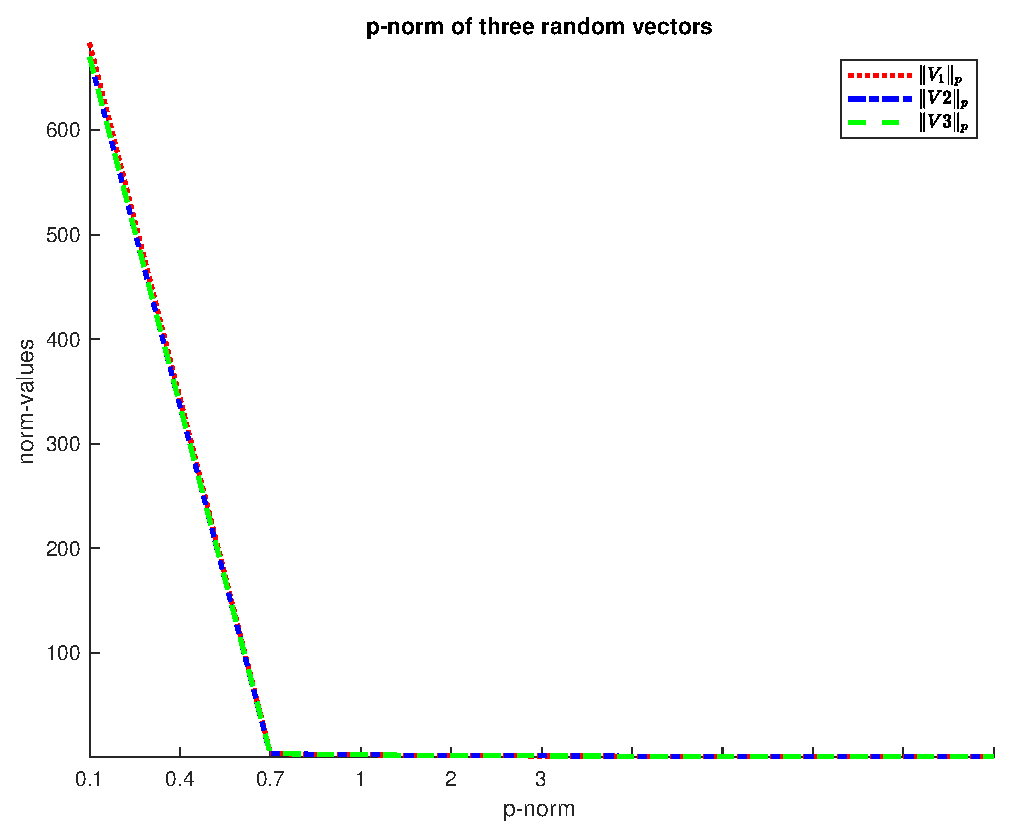
\includegraphics[width=200pt]{figures/p_norm_trend}
	\caption{p-norms of three random vectors }
	\label{fig6}
\end{figure}

%which is equivalent of solving the problem:
%\begin{align*}
%	\text{ maximize } &  r\\
%	\text{subject to }  &g_i(x, r) \le 0,  i=1, \cdots, m
%\end{align*}
%where $g_i(x, r) = \sup_{\|u\|_p \le r}{\{  a_i^T x_c + r \|a_i\|_p - b_i \}}$.
% This a convex optimization problem, since each function $g_i$ is the pointwise maximum of a family of convex functions of x and r, hence convex.


\end{enumerate}

\end{enumerate}

\end{document}
